\chapter{Opérer avec les relatifs}\label{ChOpererRelatifs}


\vspace{5cm}

\begin{acquis}
\begin{itemize}
\item additionner deux nombres relatifs;
\item additionner plusieurs nombres relatifs;
\item simplifier l’écriture d’une succession d’additions;
\item soustraire deux nombres relatifs;
\item calculer des expressions avec additions et soustractions;
\item calculer des expressions avec additions, soustractions et parenthèses (priorité);
\item résoudre des problèmes simples avec additions et soustractions.
\end{itemize}
\end{acquis}


\activites

\begin{activite}[Il faut régler l'addition !]

À la fête foraine, Mamadou a choisi un jeu comportant deux manches à l'issue desquelles il peut gagner ou perdre de l'argent. Un gain de 3 CHF est noté $+3$ ou 3 tandis qu'une perte de 7 CHF est notée $-7$.
\begin{partie}
Donne le bilan de chacune des parties suivantes :
\begin{itemize}
\item Partie 1 : Mamadou a gagné 3 CHF puis a gagné 7 CHF.
\item Partie 2 : Mamadou a gagné 8 CHF puis a perdu 5 CHF.
\item Partie 3 : Mamadou a perdu 4 CHF puis a perdu 6 CHF.
\item Partie 4 : Mamadou a perdu 9 CHF puis a gagné 2 CHF.
\end{itemize}
\end{partie}

\begin{partie}[Dans un tableau]
\begin{enumerate}
 \item Recopie le tableau ci-dessous qui représente les gains et les pertes des deux manches de plusieurs parties :
 
 \begin{center}
 \begin{tabularx}{0.95\linewidth}{|c|*{6}{>{\centering\arraybackslash}X|}}
\hline
\rowcolor{Gris2} & A & B & C & D \\ \hline
\cellcolor{Gris2} 1 & \cellcolor{J2} Partie n\up{$\circ$} & \cellcolor{J2} 1\up{ère} manche & \cellcolor{J2} 2\up{ème} manche & \cellcolor{J2} Bilan de la partie \\ \hline
\cellcolor{Gris2} 2 & \cellcolor{J2}1 & \cellcolor{J2} $+3$ & \cellcolor{J2} $+7$ & \cellcolor{H1} \\ \hline
\cellcolor{Gris2} 3 & \cellcolor{J2} 2 & \cellcolor{J2} $+8$ & \cellcolor{J2} $-5$ & \cellcolor{J2} \\ \hline
\cellcolor{Gris2} 4 & \cellcolor{J2} 3 & \cellcolor{J2} $-4$ & \cellcolor{J2} $-6$ & \cellcolor{J2} \\ \hline
\cellcolor{Gris2} 5 & \cellcolor{J2} 4 & \cellcolor{J2} $-9$ & \cellcolor{J2} $+2$ & \cellcolor{J2} \\ \hline
\cellcolor{Gris2} 6 & \cellcolor{J2} 5 & \cellcolor{J2} $-7$ & \cellcolor{J2} $+10$ & \cellcolor{J2} \\ \hline
\cellcolor{Gris2} 7 & \cellcolor{J2} 6 & \cellcolor{J2} $-3$ & \cellcolor{J2} $-9$ & \cellcolor{J2} \\ \hline
\cellcolor{Gris2} 8 & \cellcolor{J2} 7 & \cellcolor{J2} $+8$ & \cellcolor{J2} $+2$ & \cellcolor{J2} \\ \hline
\cellcolor{Gris2} 9 & \cellcolor{J2} 8 & \cellcolor{J2} $+4$ & \cellcolor{J2} $-2$ & \cellcolor{J2} \\ \hline
\cellcolor{Gris2} 10 & \cellcolor{J2} 9 & \cellcolor{J2} $+5$ & \cellcolor{J2} $-7$ & \cellcolor{J2} \\ \hline
\cellcolor{Gris2} 11 & \cellcolor{J2} 10 & \cellcolor{J2} $+10$ & \cellcolor{J2} $+12$ & \cellcolor{J2} \\ \hline
\end{tabularx}
 \end{center}

 \item Effectue les calculs des cases $D2$ à $D11$.
 \end{enumerate}
\end{partie}

\begin{partie}[Addition de deux nombres relatifs]
\begin{enumerate}
 \item Sur le tableau, colorie en rouge les parties où Mamadou a gagné ou perdu de l'argent à chacune des deux manches :
 \item Pour chaque cas, quelle opération fais-tu pour trouver la valeur absolue du bilan ? 
 \item Dans quels cas le bilan est-il positif ? négatif ?
 \item Déduis-en une règle pour additionner deux nombres relatifs de même signe.
 \item Que représentent les cas qui ne sont pas coloriés en rouge ? Dans ces cas :
 \item Quelle opération fais-tu pour trouver la valeur absolue du bilan ? 
 \item Comment détermines-tu le signe du bilan ? 
 \item Déduis-en une règle pour additionner deux nombres relatifs de signes différents. 
 \end{enumerate}
\end{partie}

\begin{partie}
Recopie et complète :
\begin{colenumerate}{3}
 \item $(+8) + (+2) = \ldots \dots$ ;
 \item $(-7) + (+5) = \ldots \dots$ ;
 \item $(-4) + (-6) = \ldots \dots$ ;
 \item $(-4) + (+7) = \ldots \dots$ ;
 \item $(-5) + (-9) = \ldots \dots$ ;
 \item $(+1) + (-4) = \ldots \dots$.
 \end{colenumerate}
\end{partie}

\end{activite}

%%%%%%%%%%%%%%%%%%%%%%%%%%%%%%%%%%%%%%%%%%%%%%%%%%%%%%%%%%%%%%%%%%%%%%

\begin{activite}[Quelles différences \ldots]

Voici un tableau qui donne les températures en degrés Celsius durant une semaine à Caprino lors d'un hiver très rigoureux :

 \begin{center}
 \begin{tabularx}{1.05\linewidth}{|c|*{8}{>{\centering\arraybackslash}X|}}
\hline
\rowcolor{J2} Jour & lundi & mardi & mercredi & jeudi & vendredi & samedi & dimanche \\ \hline
\rowcolor{J2} Température & $+2$ & $+6$ & $+3$ & $-5$ & $-7$ & $-3$ & $+1$ \\ \hline
\end{tabularx}
 \end{center}
 \vspace{-0.12cm}
 \qquad \qquad \begin{tabularx}{0.9\linewidth}{|c|*{7}{>{\centering\arraybackslash}X|}}
\hline
\rowcolor{J2} Variation & $+4$ & $-3$ & & & & \\ \hline
\end{tabularx} \\[0.5em]
La variation indique la différence de température remarquée entre deux jours consécutifs.

\begin{partie}
Complète ce tableau.

La différence de température entre le lundi et le mardi est de $+4^{\circ}$C. On peut écrire : $(+6) - (+2) = (+4)$.
\end{partie}

\begin{partie} \label{OpererRelatifs_actiA}
En utilisant les réponses du tableau précédent, complète de la même manière les différences suivantes :
\begin{colenumerate}{3}
 \item $(+6) - (+2) = (+4)$ ;
 \vspace{.5em}
 \item $(+3) - (+6) = \dots \dots$ ;
 \item $(-5) - (+3) = \dots \dots$ ;
 \item $(-7) - (-5) = \dots \dots$ ;
 \item $(-3) - (-7) = \dots \dots$ ;
 \item $(+1) - (-3) = \dots \dots$ .
 \end{colenumerate}
\end{partie}

\begin{partie}
Calcule les sommes suivantes : \label{OpererRelatifs_actiB}
\begin{colenumerate}{3}
 \item $(+6) + (-2) = (+4)$ ;
\vspace{.5em}
 \item $(+3) + (-6) = \dots \dots$ ;
 \item $(-5) + (-3) = \dots \dots$ ;
 \item $(-7) + (+5) = \dots \dots$ ;
 \item $(-3) + (+7) = \dots \dots$ ;
 \item $(+1) + (+3) = \dots \dots$ .
 \end{colenumerate}
\end{partie}

\begin{partie}
Compare les calculs et les résultats des parties \ref{OpererRelatifs_actiA} et \ref{OpererRelatifs_actiB}. Que remarques-tu ?

Complète la phrase suivante :

« Soustraire un nombre relatif revient à \ldots \ldots \ldots \ldots ~son~  \ldots \ldots \ldots \ldots . »
\end{partie}

\begin{partie}
Effectue les soustractions suivantes en transformant d'abord chaque soustraction en addition :
\vspace{0.1em}
\begin{colenumerate}{1}
 \item $(+7) - (+11) =$ \dotfill;
\vspace{0.5em}
 \item $(+29) - (-15) =$ \dotfill;
 \vspace{0.5em}
 \item $(-73) - (-52) =$ \dotfill.
 \end{colenumerate}
\end{partie}

\end{activite}


%%%%%%%%%%%%%%%%%%%%%%%%%%%%%%%%%%%%%%%%%%%%%%%%%%%%%%%%%%%%%%%%%%%%%
%%%%%%%%%%%%%%%%%%%%%%%%%%%%%%%%%%%
%%%%%%%%%%%%%%%%%%%%%%%%%%%%%%%%%%%
%MiseEnPage
%%%%%%%%%%%%%%%%%%%%%%%%%%%%%%%%%%%
\newpage
%%%%%%%%%%%%%%%%%%%%%%%%%%%%%%%%%%%
%%%%%%%%%%%%%%%%%%%%%%%%%%%%%%%%%%%

\begin{activite}[Pour tout simplifier]

\begin{partie}[Simplification, 1\up{er} acte]
\begin{enumerate}
 \item Effectue les calculs $(+6) + (-4)$ et $6 - 4$. Que remarques-tu ?
 \item Simplifie de même l'écriture de $(+7) + (-1)$ puis effectue le calcul.
 \end{enumerate}
\end{partie}

\begin{partie}[Simplification, 2\up{ème} acte]
\begin{enumerate}
 \item Effectue les calculs $(+7) - (+5)$ et $7 -  5$. Que remarques-tu ?
 \item Simplifie de même l'écriture de $(+12) - (+7)$ puis calcule.
 \end{enumerate}
\end{partie}

\begin{partie}[Simplification, 3\up{ème} acte]
\begin{enumerate}
 \item Effectue $(-10) + (+1)$.
 \item Pour soustraire 9 à un nombre, il est souvent plus rapide de soustraire 10 puis d'ajouter 1, ce qu'on peut noter : $-10 + 1 = \ldots$ . Qu'en déduis-tu ?
 \end{enumerate}
\end{partie}

\begin{partie}[Simplification, dernier acte]
\begin{enumerate}
 \item Effectue les calculs $(-9) - (-2)$ et $-9 + 2$. Que remarques-tu ?
 \item Simplifie alors l'écriture de $(+8) - (-7)$ puis calcule.
 \end{enumerate}
\end{partie}

\begin{partie}
En observant bien les questions précédentes, essaie de supprimer les parenthèses et les signes inutiles dans l'expression :  $A = (-5) + (-9) - (+3)$ puis effectue le calcul.

\end{partie}


\end{activite}



\exercicesbase
\begin{colonne*exercice}

\serie{Sommes de relatifs}

\begin{exercice}
Recopie dans ton cahier, effectue les additions puis relie chaque calcul à son résultat :
\begin{center}
 \begin{tabularx}{0.95\linewidth}{|cc|X|cc|}
  \cline{1-2}\cline{4-5}
  $(-12) + (-4)$ & $\cdot$ & & $\cdot$ & $+4$ \\ \cline{1-2}\cline{4-5}
  $(+12) + (-4)$ & $\cdot$ & & $\cdot$ & $-20$ \\ \cline{1-2}\cline{4-5}
  $(-12) + (-8)$ & $\cdot$ & & $\cdot$ & $-16$ \\ \cline{1-2}\cline{4-5}
  $(-8) + (+12)$ & $\cdot$ & & $\cdot$ & $+12$ \\ \cline{1-2}\cline{4-5}
  $(+8) + (+4)$ & $\cdot$ & & $\cdot$ & $+8$ \\ \cline{1-2}\cline{4-5}
  \end{tabularx}
  \end{center}
\end{exercice}

\begin{exercice}
Effectue les additions suivantes :
\begin{colenumerate}{2}
 \item $(+2) + (+7)=$ \dotfill;
 \vspace{.3em}
 \item $(-4) + (+5)=$ \dotfill;
 \vspace{.3em}
 \item $(-8) + (-14)=$ \dotfill;
  \vspace{.3em}
 \item $(+9) + (-9)=$ \dotfill;
  \vspace{.3em}
 \item $(-20) + (-12)=$ \dotfill;
  \vspace{.3em}
 \item $(+40) + (-60)=$ \dotfill;
  \vspace{.3em}
 \item $(-36) + (+18)=$ \dotfill;
  \vspace{.3em}
 \item $(-25) + (+0)=$\dotfill.
 \end{colenumerate}
\end{exercice}


\begin{exercice}
Effectue les additions suivantes :
\begin{enumerate}
 \item $(-8) + (-16)=$ \dotfill;
   \vspace{.3em}
 \item $(+24) + (-4)=$ \dotfill;
    \vspace{.3em}
 \item $(-14) + (-3)=$ \dotfill;
    \vspace{.3em}
 \item $(-7) + (+7)=$ \dotfill;
    \vspace{.3em}
 \item $(+14) + (+8)=$ \dotfill;
    \vspace{.3em}
 \item $(+11) + (+33)=$ \dotfill;
    \vspace{.3em}
 \item $(+30) + (-47)=$ \dotfill;
    \vspace{.3em}
 \item $(+19) + (+1)=$ \dotfill;
    \vspace{.3em}
 \item $(-11) + (-13)=$ \dotfill;
    \vspace{.3em}
 \item $(+63) + (-63)=$\dotfill.
 \end{enumerate}
\end{exercice}


\begin{exercice}
Effectue les additions suivantes :
\begin{colenumerate}{1}
 \item $(-2,3) + (-4,7)=$ \dotfill ;
    \vspace{.3em}
 \item $(+6,8) + (-9,9)=$ \dotfill;
    \vspace{.3em}
 \item $(-3,5) + (+1,8)=$ \dotfill;
    \vspace{.3em}
 \item $(-2,51) + (-0)=$ \dotfill;
    \vspace{.3em}
 \item $(-7,8) + (-2,1)=$ \dotfill;
    \vspace{.3em}
 \item $(+13,4) + (-20,7)=$ \dotfill;
    \vspace{.3em}
 \item $(-10,8) + (+11,2)=$ \dotfill;
    \vspace{.3em}
 \item $(+17) + (+5,47)=$\dotfill.
 \end{colenumerate}
\end{exercice}


\begin{exercice}[La pyramide]
Recopie puis complète les pyramides suivantes sachant que le nombre contenu dans une case est la somme des nombres contenus dans les deux cases situées en dessous de lui : \\

\begin{minipage}[c]{0.48\linewidth}
\begin{center} 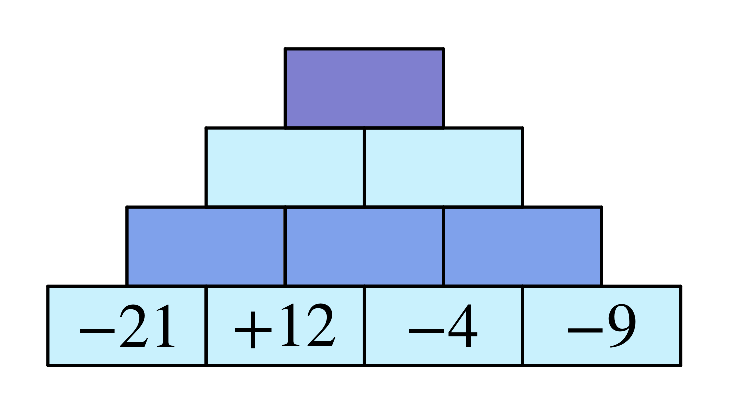
\includegraphics[width=4cm]{pyramide1_OpererRelatifs} \end{center}
\end{minipage} \hfill%
 \begin{minipage}[c]{0.48\linewidth}
\begin{center} 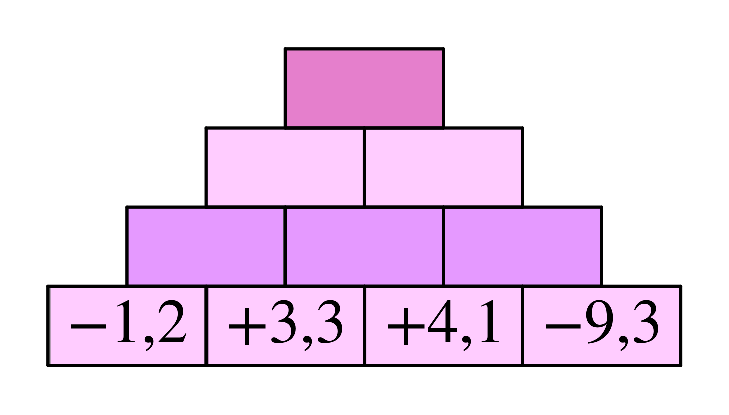
\includegraphics[width=4cm]{pyramide2_OpererRelatifs} \end{center} 
\end{minipage} \\
\end{exercice}


\begin{exercice}[La pyramide (bis)]
\vspace{0.5em}
\begin{minipage}[c]{0.48\linewidth}
\begin{center} 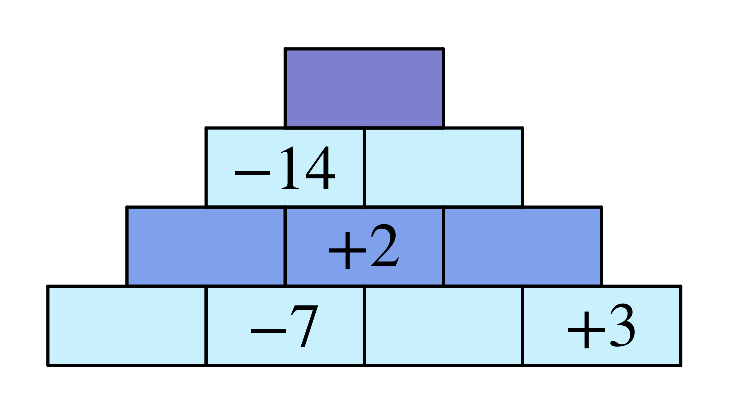
\includegraphics[width=3.8cm]{pyramide3_OpererRelatifs} \end{center}
 \end{minipage} \hfill%
 \begin{minipage}[c]{0.48\linewidth}
\begin{center} 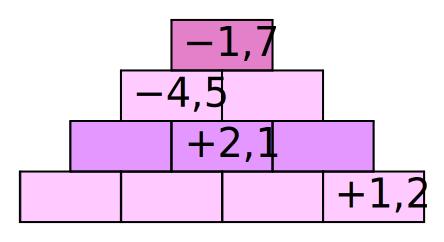
\includegraphics[width=3.8cm]{pyramide4_OpererRelatifs} \end{center}
  \end{minipage} \\
\end{exercice}


\begin{exercice}
Effectue les additions suivantes en détail :
\begin{enumerate}
 \item $(+3) + (-7) + (-8) + (+2)$ ;
 \item $(-9) + (-14) + (+25) + (-3)$ ;
 \item $(-2,3) + (-12,7) + (+24,7) + (-1,01)$ ;
 \item $(+7,8) + (+2,35) + (-9,55) + (+4)$.
 \end{enumerate}
\end{exercice}


\begin{exercice}
Calcule les sommes suivantes en détail :
\begin{enumerate}
 \item $(+17) + (-5) + (+4) + (+5) + (-3)$ ;
 \item $(-12) + (-4) + (+7) + (+8) + (-6)$ ;
 \item $(-3) + (+5) + (-4) + (+6) + (-1)$ ;
 \item $(+1,2) + (-4,2) + (+7,1) + (-6,7)$.
 \end{enumerate}
\end{exercice}


\begin{exercice}[Durées de vie]
Remarque : pour cet exercice, n'oubliez pas que l'an 0 n'existe pas.
\begin{enumerate}
 \item Cicéron est né en l'an $-23$ et est mort en l'an 38. Combien de temps a-t-il vécu ?
 \item Thalès de Milet est né en l'an $-625$ et est mort à l'âge de 78 ans. En quelle année est-il mort ?
 \item L'Empire de Césarius a été créé en $-330$ et s'est terminé en 213. Combien de temps a-t-il duré ?
 \item Ératosthène est mort en l'an $-194$ à l'âge de 82 ans. En quelle année est-il né ?
 \item Thésée avait 11 ans à la mort de Claudius. Claudius est mort en l'an $-18$. Thésée est mort en l'an 31. À quel âge est mort Thésée ?
 \end{enumerate}
\end{exercice}

%%%%%%%%%%%%%%%%%%%%%%%%%%%%%%%%%%%%%%%%%%%%%%%%%%%%%%%%%%%%%%%%%%%

%%%%%%%%%%%%%%%%%%%%%%%%%%%%%%%%%%%
%MiseEnPage
%%%%%%%%%%%%%%%%%%%%%%%%%%%%%%%%%%%
\newpage
%%%%%%%%%%%%%%%%%%%%%%%%%%%%%%%%%%%

\serie{Différences de relatifs}

\begin{exercice}
Complète afin de transformer les soustractions suivantes en additions :
\begin{enumerate}
 \item $(+2) - (+7) = (+2) + (\ldots \ldots)$ ;
 \item $(-4) - (+5) = (-4) + (\ldots \ldots)$ ;
 \item $(-8) - (-14) =  (\ldots \ldots) + (\ldots \ldots)$ ;
 \item $(+9) - (-9) =  (\ldots \ldots) + (\ldots \ldots)$.
 \end{enumerate}
\end{exercice}

\begin{exercice}
Transforme les soustractions suivantes en additions puis effectue-les :
\begin{colenumerate}{1}
 \item $(+4) - (+15)$ \dotfill;
 \vspace{0.4em}
 \item $(-12) - (+5)$ \dotfill;
 \vspace{0.4em}
 \item $(-10) - (-7)$ \dotfill;
 \vspace{0.4em}
 \item $(+14) - (-4)$ \dotfill;
 \vspace{0.4em}
 \item $(+6) - (+6)$ \dotfill;
 \vspace{0.4em}
 \item $(-20) - (+7)$\dotfill.
 \end{colenumerate}
\end{exercice}


\begin{exercice}
Effectue les soustractions suivantes :
\begin{colenumerate}{1}
 \item $(-2,6) - (+7,8)$ \dotfill;
 \vspace{0.4em}
 \item $(+6,4) - (+23,4)$ \dotfill;
 \vspace{0.4em}
 \item $(+4,5) - (-12,8)$ \dotfill;
 \vspace{0.4em}
 \item $(-2,7) - (-9,9)$ \dotfill;
 \vspace{0.4em}
 \item $(-12,8) - (+9,5)$ \dotfill;
 \vspace{0.4em}
 \item $(+6,7) - (+2,4)$ \dotfill;
 \vspace{0.4em}
 \item $(+8,1) - (-13,6)$ \dotfill;
 \vspace{0.4em}
 \item $(-12,7) - (-9,8)$\dotfill.
 \end{colenumerate}
\end{exercice}


\begin{exercice}
Pour chaque expression, transforme les soustractions en additions puis effectue les calculs :
\begin{enumerate}
 \item $(+4) - (-2) + (-8) - (+7)$ ;
 \item $(-27) - (-35) - (-20) + (+17)$ ;
 \item $(+3,1) + (-3,5) - (+7,8) - (+1,6)$ ;
 \item $(-16,1) - (+4,25) + (+7,85) - (+1,66)$.
 \end{enumerate}
\end{exercice}


\begin{exercice}
Jean et Saïd vont à la fête foraine. Ils misent la même somme d'argent au départ. Jean perd 2,30 CHF puis gagne 7,10 CHF. Saïd gagne 6 CHF puis perd 1,30 CHF. Lequel des deux amis a remporté le plus d'argent à la fin du jeu ?
\end{exercice}

%%%%%%%%%%%%%%%%%%%%%%%%%%%%%%%%%%%
%MiseEnPage
%%%%%%%%%%%%%%%%%%%%%%%%%%%%%%%%%%%
\columnbreak
%%%%%%%%%%%%%%%%%%%%%%%%%%%%%%%%%%%


\begin{exercice}
Pour chaque expression, transforme les soustractions en additions puis calcule les sommes :
\begin{enumerate}
 \item $(+12) - (-6) + (-2) + (+7) - (+8)$ ;
 \item $(-20) - (+14) + (+40) + (-12) - (-10)$ ;
 \item $(-2,4) + (-7,1) - (-3,2) - (+1,5) + (+8,4)$ ;
 \item $(+1,9) - (-6,8) + (-10,4) + (+7,7) - (+2)$.
 \end{enumerate}
\end{exercice}


\begin{exercice}
Le professeur Sésamatheux donne à ses élèves un questionnaire à choix multiples (Q.C.M) comportant huit questions. Il note de la façon suivante :
\begin{itemize}
 \item Réponse fausse ($F$) : $-3$
 \item Sans réponse ($S$) : $-1$
 \item Réponse bonne ($B$) : $+4$
 \end{itemize}
 \vspace{-0.4em}
 \begin{enumerate}
 \item Calcule la note de Wenda dont les résultats aux questions sont : $F$ ; $B$ ; $S$ ; $F$ ; $F$ ; $B$ ; $B$ ; $S$. 
 \item Quelle est la note la plus basse qu'un élève peut obtenir ? Et la plus haute ?
 \item Quels sont les résultats possibles pour Emeline qui a obtenu une note $+4$ ?
 \end{enumerate}
\end{exercice}


\begin{exercice}
Calcule astucieusement les expressions suivantes :
\begin{enumerate}
 \item $(+14) + (-45) + (-14) + (+15)$ ;
 \item $(-1,4) + (-1,2) + (+1,6) - (+1,6)$ ;
 \item $(+1,35) + (-2,7) - (-0,65) + (-1,3)$ ;
 \item $(-5,45) - (-0,45) + (+1,3) - (-1) - (+1,3)$.
 \end{enumerate}
\end{exercice}


\begin{exercice}
Remplace les pointillés par le nombre qui convient :
\begin{enumerate}
 \item $(-10) - \ldots \ldots  = 25$ ;
 \item $(+16) - \ldots \ldots  = 42$ ;
 \item $(+25) - (-13) + (-5) + \ldots \ldots = 26$ ;
 \item $(-63) + (-8) - \ldots \ldots + (+18) = 21$.
 \end{enumerate}
\end{exercice}


\begin{exercice}
Pour chaque cas, calcule en détail $x + y - z$ et $x - (y + z)$ :
\begin{center}
\begin{tabularx}{0.4\linewidth}{|X|c|c|c|}
\hline
 & x & y & z \\ \hline
\textbf{a.} & 10 & $-3$ & 8 \\ \hline
\textbf{b.} & $-6$ & $-5$ & 2 \\ \hline
\textbf{c.} & 3 & $-8$ & $-2$ \\ \hline
\textbf{d.} & 7 & $-2$ & $-5$ \\ \hline
 \end{tabularx}
 \end{center}
\end{exercice}

%%%%%%%%%%%%%%%%%%%%%%%%%%%%%%%%%%%%%%%%%%%%%%%%%%%%%%%%%%%%%%%%%%%
%%%%%%%%%%%%%%%%%%%%%%%%%%%%%%%%%%%
%MiseEnPage
%%%%%%%%%%%%%%%%%%%%%%%%%%%%%%%%%%%
\newpage
%%%%%%%%%%%%%%%%%%%%%%%%%%%%%%%%%%%


\serie{Écriture simplifiée}

\begin{exercice}
Relie chaque expression à son écriture simplifiée :
\begin{center}
 \begin{tabularx}{0.8\linewidth}{|cc|X|cc|}
  \cline{1-2}\cline{4-5}
  $(-8) + (-16)$ & $\bullet$ & & $\bullet$ & $-14 - 3$ \\ \cline{1-2}\cline{4-5}
  $(+24) - (-4)$ & $\bullet$ & & $\bullet$ & $-8 - 16$ \\ \cline{1-2}\cline{4-5}
  $(-14) + (-3)$ & $\bullet$ & & $\bullet$ & $14 + 8$ \\ \cline{1-2}\cline{4-5}
  $(-7) - (+7)$ & $\bullet$ & & $\bullet$ & $-7 - 7$ \\ \cline{1-2}\cline{4-5}
  $(+14) + (+8)$ & $\bullet$ & & $\bullet$ & $24 + 4$ \\ \cline{1-2}\cline{4-5}
  \end{tabularx}
  \end{center}
\end{exercice}


\begin{exercice}
Recopie et complète le tableau :
\begin{center}
\begin{tabularx}{0.98\linewidth}{|c|X|c|}

\hline
 & Écriture avec & Écriture simplifiée \\ 
  & parenthèses &  \\ \hline

\textbf{a.} & \footnotesize{$(-9) - (+13) + (-15)$} & \\ \hline
\textbf{b.} & \footnotesize{$(-10) + (+7) - (-3) - (-3)$} & \\ \hline
\textbf{c.} & \footnotesize{$(+5) - (-2) + (+3) - (+2)$} & \\ \hline
\textbf{d.} & & \footnotesize{$-6 - 8 + 5 - 3$} \\ \hline
\textbf{e.} & & \footnotesize{$15 - 13 - 8 - 7$} \\ \hline
\textbf{f.} & & \footnotesize{$-13 - 5 - 9 + 1$} \\ \hline
 \end{tabularx}
 \end{center}
\end{exercice}


\begin{exercice}
Donne une écriture simplifiée des expressions suivantes en supprimant les parenthèses et les signes qui ne sont pas nécessaires:
\begin{enumerate}
 \item $(-5) + (-3)$ ;
 \item $(-4) - (+6)$ ;
 \item $(+9) - (-3)$ ;
 \item $(+4) + (+7)$ ;
  \item $(+17) - (-5) + (+4) - (+5) - (-3)$ ;
  \item $(-15) + (+3,5) - (-7,9) + (-13,6)$.
  \end{enumerate}
\end{exercice}


\begin{exercice}
Effectue les calculs suivants :
\begin{colenumerate}{2}
 \item $5 - 14$ ;
 \item $8 - 13$ ;
 \item $-6 - 6$ ;
 \item $-13 + 9$ ;
 \item $-53 - 48$ ;
 \item $-2,8 - 4,7$ ;
 \item $-5,7 + 4,4$ ;
 \item $3,2 - 8,9$.
 \end{colenumerate}
\end{exercice}


\begin{exercice}
Effectue en détail :
\begin{colenumerate}{2}
 \item $24 - 36 + 18$ ;
 \item $-13 - 28 + 35$ ;
 \item $-3,8 - 4,4 + 8,2$ ;
 \item $18 - 8 + 4 - 14$ ;
 \item $-1,3 + 4,4 - 21$ ;
 \item $14 - 23 + 56 - 33$.
 \end{colenumerate}
\end{exercice}


\begin{exercice}
Effectue en détail :
\begin{enumerate}
 \item $5 + 13 - 4 + 3 - 6$ ;
 \item $-7 + 5 - 4 - 8 + 13$ ;
 \item $3,5 - 4,2 + 6,5 - 3,5 + 5$ ;
 \item $25,2 + 12 - 4,8 + 24 - 3,4$.
 \end{enumerate}
\end{exercice}


\begin{exercice}
Regroupe les termes astucieusement puis effectue en détail :
\begin{enumerate}
 \item $13 + 15 + 7 - 15$ ;
 \item $-8 + 4 + 18 - 2 + 12 + 6$ ;
 \item $4,3 - 7,4 + 4 - 2,25 + 6,7 + 3,4 - 2,75$ ;
 \item $-2,5 + 4,8 - 3,6 + 0,2 + 2,5$.
 \end{enumerate}
\end{exercice}


\begin{exercice}
Calcule les expressions suivantes, en détail :
\begin{enumerate}
 \item $(-3 + 9) - (4 - 11) - (-5 - 6)$ ;
 \item $-3 + 12 - (13 - 8) - (3 + 8)$ ;
 \item $-3 - [4 - (3 - 9)]$.
 \end{enumerate}
\end{exercice}


\begin{exercice}[Températures]
Pour mesurer la température, il existe plusieurs unités. Celle que nous utilisons en Suisse est le degré Celsius ($^{\circ}$C). Cette unité est faite de façon à ce que la température à laquelle l'eau se transforme en glace est $0^{\circ}$C et celle à laquelle l'eau se transforme en vapeur est $100^{\circ}$C. Dans cette échelle, il existe des températures négatives. \\[0.5em]
Il existe une autre unité, le Kelvin (K), dans laquelle les températures négatives n'existent pas. Pour passer de l'une à l'autre, on utilise la formule :
\begin{center} $T_\text{Kelvin} = T_\text{degrés Celsius} + 273,15$ \end{center}
Ainsi, $10^{\circ}$C correspondent à 283,15 K.
\begin{enumerate}
 \item Convertis en Kelvin les températures suivantes : $24^{\circ}$C ; $-3^{\circ}$C et $-22,7^{\circ}$C ;
 \item Convertis en degré Celsius les températures suivantes : 127,7 K ; 276,83 K ; 204 K et 500 K ;
 \item Quelle est en Kelvin la plus petite température possible ? À quelle température en degré Celsius correspond-elle ? Cette température est appelée le zéro absolu.
 \end{enumerate}
\end{exercice}

\end{colonne*exercice}


\exercicesappr
\begin{colonne*exercice}
\begin{exercice}[Sur un axe gradué]
\begin{enumerate}
 \item Soit $A$ le point d'abscisse 4. Quelle peut-être l'abscisse du point $B$ sachant que la longueur du segment $[AB] = 8$ ?
 \item Soit $C$ le point d'abscisse $-3$. Quelle peut-être l'abscisse du point $D$ sachant que la longueur du segment $[CD] = 2$ ?
 \item Soit $E$ le point d'abscisse $-5$. Détermine l'abscisse de $F$ sachant que la longueur du segment $[EF] = 9$ et que l'abscisse de $F$ est inférieure à celle de $E$.
 \end{enumerate}
\end{exercice}


\begin{exercice}
Recopie en remplaçant les $\lozenge$ par le signe $-$ ou le signe $+$ de sorte que les égalités soient vraies :
\begin{enumerate}
 \item $\lozenge \quad 7 \quad \lozenge \quad 3 = -4$ ;
 \item $\lozenge \quad 13 \quad \lozenge \quad 8 = -21$ ;
 \item $\lozenge \quad 3,7 \quad \lozenge \quad 8,4 = 4,7$ ;
 \item $\lozenge \quad 45 \quad \lozenge \quad 72 = -27$ ;
 \item $\lozenge \quad 2 \quad \lozenge \quad 7 \quad \lozenge \quad 13 = -8$ ;
 \item $\lozenge \quad 1,5 \quad \lozenge \quad 2,3 \quad \lozenge \quad 4,9 = -5,7$ ;
 \item $\lozenge \quad 8 \quad \lozenge \quad 5 \quad \lozenge \quad 12 \quad \lozenge \quad 2 = 13$ ;
 \item $\lozenge \quad 7 \quad \lozenge \quad 14 \quad \lozenge \quad 18 \quad \lozenge \quad 3 = -22$.
 \end{enumerate}
\end{exercice}


\begin{exercice}[Carré magique]
Recopie et complète ce carré magique sachant qu'il contient tous les entiers de $- 12$ à $12$ et que les sommes des nombres de chaque ligne, de chaque colonne et de chaque diagonale sont toutes nulles :
\begin{center}
\begin{tabular}{|*5{@{}>{\vrule width0pt height\dimexpr1cm/2+1ex-.2pt\relax depth\dimexpr1cm/2-1ex-.2pt\relax\centering\arraybackslash}p{\dimexpr1cm-.4pt\relax}@{}|}}\hline
    & & 0 & 8 & \\\hline
    & & & $-11$ & 2 \\\hline
   $-9$ & $-1$ & 12 & & 3 \\\hline
   $-3$ & & $-12$ & & 9 \\\hline
   $-2$ & 11 & $-6$ & 7 & \\\hline
\end{tabular}
 \end{center}
\end{exercice}


\begin{exercice}[Triangle magique]
La somme des nombres de chaque côté du triangle est 2. Remplis les cases vides avec les nombres relatifs $(-2)$ ; $(-1)$ ; 1 ; 2 et 3, qui doivent tous être utilisés.
\end{exercice}


\begin{exercice}[Coup de froid]
Chaque matin de la 1\up{re} semaine du mois de Février, Julie a relevé la température extérieure puis a construit le tableau suivant :
\begin{center}
\begin{tabularx}{1.03\linewidth}{|c|*{8}{>{\centering \arraybackslash}X|}}
\hline \cellcolor{H1} Jour & \cellcolor{H2} \small{Lu} & \cellcolor{H2} \small{Ma} & \cellcolor{H2} \small{Me} & \cellcolor{H2} \small{Je} & \cellcolor{H2} \small{Ve} & \cellcolor{H2} \small{Sa} & \cellcolor{H2} \small{Di} \\
\hline \cellcolor{U1} \small{Température (en $^{\circ}$C)} & \cellcolor{U2} \small{$-4$} & \cellcolor{U2} \small{$-2$} & \cellcolor{U2} \small{$-1$} & \cellcolor{U2} \small{$+1$} & \cellcolor{U2} \small{0} & \cellcolor{U2} \small{$+2$} & \cellcolor{U2} \small{$-3$} \\
\hline
\end{tabularx} \\
\end{center}
Calcule la moyenne des températures relevées par Julie.
\end{exercice}


\begin{exercice}
Recopie et complète les carrés magiques suivants :
\begin{enumerate}
 \item Pour l'addition : \\[0.5em]
\begin{center}
\begin{tabular}{|*3{@{}>{\vrule width0pt height\dimexpr1cm/2+1ex-.2pt\relax depth\dimexpr1cm/2-1ex-.2pt\relax\centering\arraybackslash}p{\dimexpr1cm-.4pt\relax}@{}|}}\hline
 &  $-9$ &  $-2$ \\ \hline
 &  $-4$ &  \\ \hline
 $-6$ &  &  \\ \hline
\end{tabular}
\end{center}
\vspace{0.5cm}
 \item Pour l'addition : \\[0.5em]
 \begin{center}
\begin{tabular}{|*3{@{}>{\vrule width0pt height\dimexpr1.4cm/2+1ex-.2pt\relax depth\dimexpr1.4cm/2-1ex-.2pt\relax\centering\arraybackslash}p{\dimexpr1.4cm-.4pt\relax}@{}|}}\hline
 1,6 &  &  \\ \hline
 &  $-5,4$ &  \\ \hline
 $-4,4$ &  &  $-12,4$\\ \hline
\end{tabular}
\end{center}
 \end{enumerate}
\end{exercice}


\begin{exercice}
La différence $a - b$ est égale à 12.

On augmente $a$ de 3 et on diminue $b$ de 4.

Combien vaut la différence entre ces deux nouveaux nombres? 
\end{exercice}


\begin{exercice}[Le nombre $-21$...]
\begin{enumerate}
 \item Écris le nombre $-21$ comme somme de deux nombres entiers relatifs consécutifs ;
 \item Écris le nombre $-21$ comme différence de deux carrés.
 \end{enumerate}
\end{exercice}



\end{colonne*exercice}

\connaissances


\QCMautoevaluation{Pour chaque question, plusieurs réponses sont
  proposées. Déterminer celles qui sont correctes.}

\begin{QCM}
  \begin{GroupeQCM}
    \begin{exercice}
      $(-10) + (+15) = \ldots$
      \begin{ChoixQCM}{4}
      \item $(-5)$
      \item $(-150)$
      \item $(+5)$
      \item $(-25)$
      \end{ChoixQCM}
\begin{corrige}
     \reponseQCM{c} 
   \end{corrige}
    \end{exercice}
    
    
    \begin{exercice}
      $(+8) + \ldots = -5$
      \begin{ChoixQCM}{4}
      \item $(+3)$
      \item impossible
      \item $(+13)$
      \item $(-13)$
      \end{ChoixQCM}
\begin{corrige}
     \reponseQCM{d}
   \end{corrige}
    \end{exercice}


    \begin{exercice}
      $(+2,1) + (-3,9) = \ldots$
      \begin{ChoixQCM}{4}
      \item $6$
      \item $-6$
      \item $-1,8$
      \item $1,8$
      \end{ChoixQCM}
\begin{corrige}
     \reponseQCM{c}
   \end{corrige}
    \end{exercice}


    \begin{exercice}
      $(+7) - (-3) = \ldots$
      \begin{ChoixQCM}{4}
      \item $4$
      \item $10$
      \item $-4$
      \item $-10$
      \end{ChoixQCM}
\begin{corrige}
     \reponseQCM{b}
   \end{corrige}
    \end{exercice}


    \begin{exercice}
      $(-2) - \ldots = -5$
      \begin{ChoixQCM}{4}
      \item $(+3)$
      \item $(-7)$
      \item $(+7)$
      \item $(-3)$
      \end{ChoixQCM}
\begin{corrige}
     \reponseQCM{a}
   \end{corrige}
    \end{exercice}


    \begin{exercice}
      $1,3 - (-2,4) = \ldots$
      \begin{ChoixQCM}{4}
      \item $-1,1$
      \item $1,1$
      \item $3,7$
      \item $-3,7$
      \end{ChoixQCM}
\begin{corrige}
     \reponseQCM{c}
   \end{corrige}
    \end{exercice}


\end{GroupeQCM}
\end{QCM}

%%%%%%%%%%%%%%%%%%%%%%%%%%%%%%%%%%%
%%%%%%%%%%%%%%%%%%%%%%%%%%%%%%%%%%%
%MiseEnPage
%%%%%%%%%%%%%%%%%%%%%%%%%%%%%%%%%%%
\vfill
%%%%%%%%%%%%%%%%%%%%%%%%%%%%%%%%%%%
%%%%%%%%%%%%%%%%%%%%%%%%%%%%%%%%%%%


%\TravauxPratiques % pour nous "travailler en groupe"
%
\begin{TP}[]

Mon super TP

\end{TP}



\pagebreak

%\recreation
%\begin{enigme}[Des discontinuités... en continu !]


Soit $x$ et $y$ deux réels tels que $x<y$.\\
Définissons la suite  $(d_n)_{n\geqslant0}$ telle que $d_n=\dfrac{\lfloor10^n y\rfloor}{10^n}$ où $\lfloor a\rfloor$ désigne la partie entière de $a$.\\
\begin{enumerate}
\item À quel ensemble les nombres $d_n$  appartiennent-ils ? \hspace{1cm}
\begin{minipage}{0.5\linewidth}
\begin{colitemize}{5}
\item $\mathbb{N}$ ? \item $\mathbb{Z}$ ? \item $\mathbb{D}$ ? \item $\mathbb{Q}$ ? \item $\mathbb{R}$ ?
\end{colitemize}
\end{minipage}
\item
\begin{enumerate}
\item Montrer  que pour tout $n\in\mathbb{N}$, on a l'encadrement $\dfrac{10^ny-1}{10^n}< d_n\leqslant y$.
\item En déduire $\displaystyle\lim_{n\to+\infty}d_n$.
\end{enumerate}
\item \begin{enumerate}
\item Montrer que, quel que soit $\varepsilon>0$, il existe un entier naturel $N$ tel que pour tout $n\geqslant N$, $|d_n-y|< \varepsilon$.
\item En posant $\varepsilon=y-x$, en déduire que $x\leqslant d_N \leqslant y$.
\end{enumerate}
\end{enumerate}

\begin{center}
\begin{minipage}{1\linewidth}
\begin{cadre}[A1][A4]
On vient de montrer qu'entre deux réels, il existe toujours un décimal et donc toujours un rationnel.\\
On dit que l'ensemble des rationnels $\mathbb{Q}$ est \textbf{dense} dans l'ensemble des réels $\mathbb{R}$.
 \end{cadre}
\end{minipage}
\end{center}

La \textbf{fonction de Dirichlet} D et la \textbf{fonction de Thomae} T sont deux fonctions définies sur $\mathbb{R}$ par  :
\[\text{D}(x)=\left\{\begin{matrix} 1  &  \text{si~} x\in\mathbb{Q} \\ 0  & \text{si~} x\notin\mathbb{Q} \end{matrix}\right.
\text{~~et~~} \text{T}(x)=\left\{\begin{array}{@{}ll} 0  & \text{si~} x\notin\mathbb{Q} \\ 1 & \text{si~} x=0 \\ \dfrac{1}{q} & \text{si~} x=\dfrac{p}{q} \text{~est une fraction irréductible}\end{array}\right.\]
Introduite par Dirichlet\footnote{Johann Peter Gustav Lejeune Dirichlet (1805–1859), mathématicien allemand}  en 1829, la fonction D est discontinue partout ce que le résultat établi précédemment montre. Cette fonction est appelée aussi \textbf{fonction indicatrice des rationnels}.\\
Introduite par Thomae\footnote{Carl Johannes Thomae (1840–1921), mathématicien allemand} en 1875, la fonction T est continue en tout nombre irrationnel mais  discontinue en tout nombre rationnel. Cette fonction est appelée aussi la \textbf{fonction popcorn} (voir sa représentation ci-dessous !).
\begin{center}

\end{center}




\end{enigme} 


